\documentclass[journal]{IEEEtran}

\usepackage{cite}
\usepackage{float}
\usepackage{graphicx}
\usepackage[caption=false]{subfig}
  \DeclareGraphicsExtensions{.png}
\usepackage{amsmath}
\usepackage{amsfonts}
\usepackage{url}
\usepackage{tikz}
\usetikzlibrary{shapes,arrows}
\usepackage{bm,times}
\hyphenation{photo-graphed diff-erence}

\begin{document}

\title{%
  High radix On-line Arithmetic Verification System\\
  \large Final Year Project 1800478: Interim Report}
\author{Zifan Wang, 01077639\\Imperial College London}

% \markboth{2018-2019}{?}
\onecolumn
\maketitle
\tableofcontents

\twocolumn
\newpage
% \begin{abstract}
% \end{abstract}

% --------------------------------------------------------------------------------
% --------------------------------------------------------------------------------
\section{Introduction}
% The Interim report should normally be between 10 and 30 pages long. Remember
% that it must be a project planning document for the remainder of your project
% work, as well as being an early write-up of your background material. Using
% Interim Report material, without explicit reference, in your Final Report is
% allowed, and even encouraged. The Interim Report is often a first draft of the
% background section of the Final Report. Self-plagiarism, in this case, is not an
% issue. It is expected that you will reuse Interim Report material without
% explicit reference.
% REVISIT: this is directly from James's project discription
With the right number representation system, it is possible to perform
arithmetic operations MSD-first.
Consequently, these on-line arithmetic operators are attractive
for hardware implementation in both serial and parallel forms.
When computing digits serially, they can be chained such that subsequent
operations begin before the preceding ones complete.
Parallel implementations tend to be most sensitive to failure in their LSD,
making them more friendly to overclocking than their LSD-first counterparts,
for which the opposite is true.

In the past, online operators have typically been implemented in binary.
Along with its sister project,
This project will explore high radix on-line operators,
investigating their suitability for FPGA implementation and examining the
resultant trade-offs between performance, area and power.

\section{Background Research}
% The background section must outline the necessary background to the project,
% stating how it is important for the project work. For example: survey of related
% literature, analysis of competing products, technical specifications of hardware
% or software standards, electronic components, necessary software tools,
% background theory. The contents of this section will vary for different
% projects, and in many cases the background reading will have been completed –
% but if not you should be in a position to list what remains to be done (e.g. a
% set of research papers to read and understand). A good benchmark of progress
% here is that you have accumulated (though may not yet have read) at least 20
% references to background material. In projects which have substantial background
% writing up your literature survey in the Interim Report will save time at the
% end of the project and allow this element of your final report to receive timely
% feedback from your supervisor so the final write-up can be improved.
% REVISIT: Better logic between serial and parallel operators

\subsection{On-line Arithmetic}
Traditional proposals to achieving a faster and more efficient arithmetic
operator have two common characteristics.
One, their order operation may be different depending on the operation itself.
A traditional adder, parallel or serial, generates its answers from the LSD to
the MSD.
A traditional divider design on the other hand, generates its answers from
the MSD to the LSD~\cite{Brent1}\cite{Srinivas1}.

Due to this inconsistency, arithmetic operators may be forced to compute
word-by-word, waiting for all digits to finish in the previous operator before
moving on to the next.~\cite{Zhao1}
This means if a divider follows an adder of the same width, the divider has to
wait until the adder complete its computation before it can start its own.

The other commonality of traditional designs is that their precisions are
specified design-time. Once built, a 32-bit adder always adds 32 bits together,
as the hardware is fixed at run-time.
A possible way of making it more efficient would be using SIMD
instructions~\cite{Duncan1}, trying to combine smaller operations into a larger
one that fits the hardware.
This requires more control circuits in the hardware, or a more complex compiler.

On-line arithmetic does not suffer from the first issue as it performs all
arithmetic operations with MSD first~\cite{Ercegovac1}.
Pipelining can be used with on-line arithmetic operators.
This means the output digit of an earlier operation can be fed into the next
operator before the earlier operation been fully complete.

% REVISIT: Better diagram here
\begin{figure}[H]
  \centering
  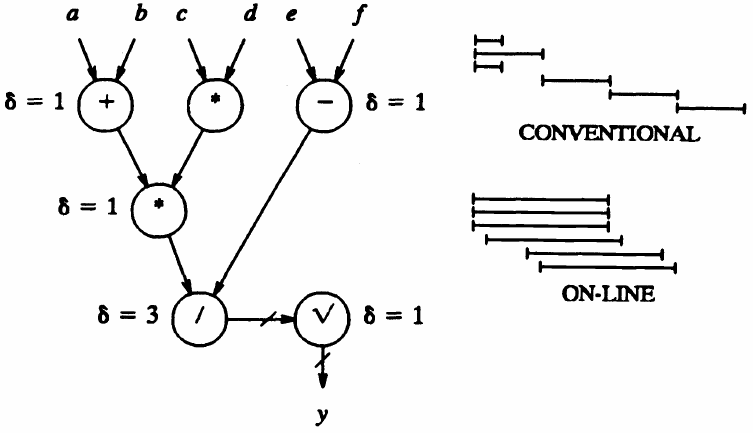
\includegraphics[width=8cm]{img/Online}
  \caption{Computing $y=\sqrt{(a+b)cd/(e-f)}$~\cite{Ercegovac1}}
  \label{Online}
\end{figure}

As illustrated in figure~\ref{Online}, while each individual operation may
take longer than its conventional counterpart, on-line arithmetic could provide
a speed up if the operators are in serial.
Individually, on-line arithmetic also sacrifices in terms of memory.
As all computation are made MSD to LSD, the use of a redundant number system
is compulsory.
However, this redundancy also has its advantage in making the operators
scalable.
The time required per digit can be made independent of the length of the
operands.~\cite{Trivedi1}

A recent architecture proposal allows the precision of
on-line arithmetic to be controlled at run-time~\cite{Zhao1}.
Traditionally, this run-time control was restricted due to the parallel adders
present in the multipliers and dividers.
This architecture reuses a fixed-precision adder and stores residues in
on-chip RAM.
As such, a single piece of hardware can be used to calculate to any precision
limited only by the size of the on-chip RAM.

Another way that on-line arithmetic alleviates the problem of fixed precision
falls out directly from its MSD-first nature.
Suppose the output of a conventional ripple adder is sampled before
it has completed its operation.
In this case, the lower digits would have been completed, but the carry would
not have reached the higher ones.
This means the error on the result would be significant, as the top bits
were still undetermined~\cite{Shi1}.

However, if the output of a serial on-line adder is sampled before its
completion, the lower bits would be the undetermined ones.
This means the error of the operation would be small.
With overclocking, on-line arithmetic would fail gracefully, losing its
precision gradually from the lowest bits first.
Thus, it allows for a run-time trade-off between precision and
frequency~\cite{Shi2}.

\subsection{High radix Arithmetic}
Conventional designs of arithmetic operators use binary representations.
This was chosen four decades ago to maximise numerical accuracy per bit of data.
However, using a high radix representation system could yield better numerical
accuracy while reducing area cost of FPGAs.
For example, a hexadecimal floating-point adder has a 30\% smaller area-time
product than its binary counterpart, while still delivering equal worst-case
and better average-case numerical accuracy~\cite{Catanzaro1}.

However, the savings are not without trade-offs.
This trade-off can become unfavourable if the specification requires much I/O
and little computation~\cite{Whyte1}.
This is because the overhead of radix conversion would be significant.
It is also unwise to use high radix representations when the numbers are
unusually small, thus making the savings offered by the high radix
negligible~\cite{Catanzaro1}.

\subsection{High radix On-line Arithmetic}
Using high radix number representations for on-line arithmetic is a
relatively novel concept.
% REVISIT: can find problem with Lynch?
While there have been some research in this field~\cite{Lynch1}\cite{Lynch2},
this project takes a more direct approach by implementing custom operators
made for high radix on-line arithmetic on a FPGA.
This would allow for empirical results to be obtained, hopefully revealing
practical insights to the method.

As an potential extension to the project, optimising this exotic arithmetic
on a system level for popular FPGA accelerations such as neural networks would
be innovative as well.
\section{Project Specification}
% The project specification should state clearly what the project is intended to
% deliver, including all hardware, software, simulation, and analytical work, and
% provide some motivation.

\subsection{Project Organisation}
This project is a part of a larger project investigating the effect of using
high-radix number representation with online arithmetic operators.
The overarching aim involves implementing such a system on an FPGA and
quantifying its performance improvements.
This is achieved through two individual projects, vertically split from
the enveloping project.
One shall design and verify the arithmetic operator modules,
while the other shall design a system from the top-level to test and
evaluate these operators.
This project deals with the system-level issues.

As this project progresses in parallel with the designing of the operator
modules, it is necessary to decouple the two projects so that, being individual
projects, they can be evaluated individually.
The success of one project should not be restricted by the status of the other.
To this end, the goal of the system-level design is more focussed on its
functionalities and robustness.
This relationship and its effect on the evaluation will be examined further in
the evaluation chapter of this report.

To ensure the two products will work together once they are both complete, a
common interface needs to be agreed upon.
The interface will be done using Qsys.
% REVISIT JD: add deliverables from Junjie
% REVISIT JD: explain interface with Qsys
% maybe just remove this sentence?
Its reasoning falls off directly from the use of the hardware;
as such it will be explained in the corresponding section.

% \subsection{Project Interfacing}
% REVISIT: project interfacing section necessary?

\subsection{Deliverables}
At the end of the project, the system should be able to perform the following:
\begin{enumerate}
  \item Connect to the arithmetic modules as its input;
  \item Generate and run tests on these modules;
  \item Vary the frequency and voltage of the FPGA;
  \item Evaluate its performance.
\end{enumerate}

\subsection{Hardware Choice}
The system itself will be built on a Cyclone V SX SoC Development Board from
Intel~\cite{Intel1}.

The 5CSXFC6D6F31C6N SoC has an Arm Cortex-A9 MPCore accompanied by Intel's 28nm
FPGA fabric~\cite{Altera1}.
The FPGA is necessary for implementing the hardware design and obtaining
empirical results for the project.
% maybe hybrid architecture soc makes programming it harder and it could
% be used as a negative point

\begin{figure}[H]
  \centering
  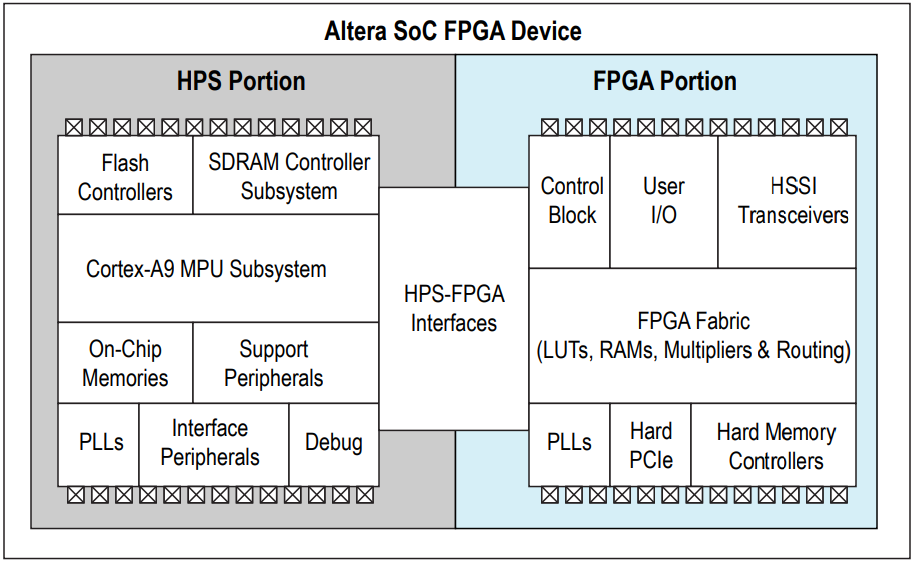
\includegraphics[width=8cm]{img/SoCStructure}
  \caption{Structure of the System-on-Chip}
  \label{SoCStructure}
\end{figure}

While an FPGA without an embedded CPU will be enough for this project to work,
having an Hard Processor System (HPS) on the same chip is useful as the test
software can run on it.
The HPS is a separate piece of hardware that distinguishes itself from a soft
processor, such as the Nios II, a processor programmed onto the FPGA itself.
With this additional capacity, a better user interface can thus be constructed
with more detailed, on-the-fly control of the FPGA.
This means setting up the testbench will only require programming the design
into the FPGA, followed by running the test script on the HPS.
The product will thus be self-contained.
It will be more accessible as no additional setup is required for the user.

It should be noted that Xilinx offers similar boards as well.
Its Zynq SoC family has a very comparable structure as they too integrate the
software programmability of an Arm processor with the hardware possibility of
an FPGA.
For example, similar to the Cyclone V SX, Zynq-7000S features an Arm Cortex-A9
coupled with a Xilinx 28nm FPGA~\cite{Xilinx1}.
As such, a board like the ZedBoard~\cite{Xilinx2} could be just as viable for
this project.

As there are very few significant functional differences between the two brands,
I shall initially explore with the Intel board, simply for its
availability and my familiarity with their development tools.
Due to the architectural differences between the logic elements between Xilinx
and Altera FPGAs~\cite{Scekic1}, the performances on the two boards are not
necessarily identical.
Once the project has progressed to a point where the system design is mature and
tested, the Xilinx alternative can be explored as an extension.

\subsection{Software Choice}
The software choice follows closely with the hardware choice in this project.
To develop for Intel FPGAs, Quartus has to be used.
The version picked is arbitrary as there are not many functional differences
between the versions that will be critical to the project.
As Quartus Prime 16.0 is the version installed in the computers in the
department, I will use the same version simply for convenience.
This naturally means the hardware system will be built with the system
integration tool that comes with Quartus -- Qsys.

The Qsys software is designed to be used for integrating different hardware
modules into a system.
As such, it will be used as the interface for the two parallel projects.

While an HLS language could be used, in this design it suffers from a few
problems and does not offer enough benefits to justify its use.
Usually HLS is preferred for developing complex algorithms, because compilers
can optimise them into RTL much better than humans.
However, the resulting RTL would be unreadable, making directly controlling or
debugging at the hardware level nearly impossible.
The interfaces require detailed control of the actual hardware and the rest of
the testbench has a lot of control path work and direct manipulation on the
data bits.
It is therefore not worth it to use HLS and as such, this design will be written
in Verilog.

Other than the hardware design tools, there is some freedom of choice on the
HPS side of the project.
The test will be built with Python, which will be running on an Ubuntu system
that is installed on the HPS.
This choice is made as there are previous unrelated projects on the same
development board, which means a lot of time can be saved on tedious setup works
such as getting an operating system booting.
\section{Engineering Background}
% REVISIT: what to put here?
% research on possible architectures
% hardware of FPGA
% speed of memory
% launch registers
% PLLs
% HLS vs Verilog?
% LFSR

\subsection{Target}
The design of the verification system is the major engineering challenge of this
project.
In order to stress the DUT, the verification system must perform at a much
higher frequency than the expected frequency of the DUT.
Assuming the DUT is to run at 300MHz, to fully explore the effect of
overclocking, the testbench must be able to run at double the frequency or
higher.
This gives a target frequency of 800MHz.
Assuming data width of 32-bits, the target data transfer rate is then 
This required data transfer rate is estimated to be 25.6Gbps.

\subsection{Data Transfer Rate}
% REVISIT: possible to find exact bandwidth of the bridge?
As the test is to be run on the HPS, the HPS-FPGA bridge will be the
immediate bottleneck if the test data is to flow from HPS to FPGA.
While HPS is able to easily generate test data,
there is a large amount of overhead as data crosses from one architecture
to another.
This overhead exists in terms of both a lowered bandwidth and a high delay.
Thus, it would not be sensible for HPS to send out data during run-time.

% --- using SDRAM
Another thought may be to first populate the off-chip DDR SDRAM on FPGA
side, then feed the data from there to the DUT during test.
This is already much faster than passing the data from HPS.
The 1GB, 32-bits wide DDR3 on FPGA side is rated at 400MHz.
With double rate transfer, this would gives a maximum transfer rate of 25.6Gbps.

While using the off-chip RAM may theoretically achieve the targets,
it still has its disadvantages.
First, the process of filling up the memory and then using them for the tests
takes time.
This means the test would be broken up into bursts with time in between for
checking the results and filling up with new data.
The complexity of the SDRAM interface also requires a SDRAM controller to be
used to manage SDRAM refresh cycles, address multiplexing and interface timing.
These all adds up to a significant access latency.
While this could be overcame with burst accesses and piplined accesses,
it would further complicate the SDRAM controller.
While this controller is provided by Altera~\cite{Altera3}, it is consumes
a non-negligible amount of the limited FPGA resources, while adding
unnecessary complexity to the design.
Customising the controller to fit this project may also be time-consuming.

% --- on-chip memory
The on-chip memory is much faster and simpler to handle.
This memory is implemented on the FPGA itself, and thus there is no external
connections for access to this memory.
It has the highest possible throughput, with the lowest possible latency
in an FPGA-based system.
The memory transactions can also be piplined, giving one transaction per
clock cycle.
With an on-chip FIFO accessed in dual-port mode, the write at one end and the
reads at the other end can happen simultaneously.
This effective doubling of the bandwidth is useful as tests are prepared
and fed into the DUT, or when test results are collected and fed to a checker.

On-chip memory is not without its drawbacks.
It is volatile and very limited in capacity.
While the off-chip can have its storage reaching 1GB, that of the on-chip
memory could only reach a few MB~\cite{Altera2}.
Volatility is not exactly of concern in this project, but its small capacity
means not much test data can be held before it needs more fed in.

Looking at the options listed above, with a way of generating test data at
run-time on the FPGA, using on-chip memory would be the most sensible option.


\subsection{Clock Domains}


\subsection{Testbench Architecture}
\newcommand{\mx}[1]{\mathbf{\bm{#1}}} % Matrix command
\newcommand{\vc}[1]{\mathbf{\bm{#1}}} % Vector command

% We need layers to draw the block diagram
\pgfdeclarelayer{background}
\pgfdeclarelayer{foreground}
\pgfsetlayers{background,main,foreground}

% Define a few styles and constants
\tikzstyle{sensor}=[draw, fill=blue!20, text width=5em, 
    text centered, minimum height=2.5em]
\tikzstyle{ann} = [above, text width=5em]
\tikzstyle{naveqs} = [sensor, text width=6em, fill=red!20, 
    minimum height=12em, rounded corners]
\def\blockdist{2.3}
\def\edgedist{2.5}

\begin{tikzpicture}
    \node (naveq) [naveqs] {Navigation equations};
    % Note the use of \path instead of \node at ... below. 
    \path (naveq.140)+(-\blockdist,0) node (gyros) [sensor] {Gyros};
    \path (naveq.-150)+(-\blockdist,0) node (accel) [sensor] {Accelero-meters};
    
    % Unfortunately we cant use the convenient \path (fromnode) -- (tonode) 
    % syntax here. This is because TikZ draws the path from the node centers
    % and clip the path at the node boundaries. We want horizontal lines, but
    % the sensor and naveq blocks aren't aligned horizontally. Instead we use
    % the line intersection syntax |- to calculate the correct coordinate
    \path [draw, ->] (gyros) -- node [above] {$\vc{\omega}_{ib}^b$} 
        (naveq.west |- gyros) ;
    % We could simply have written (gyros) .. (naveq.140). However, it's
    % best to avoid hard coding coordinates
    \path [draw, ->] (accel) -- node [above] {$\vc{f}^b$} 
        (naveq.west |- accel);
    \node (IMU) [below of=accel] {IMU};
    \path (naveq.south west)+(-0.6,-0.4) node (INS) {INS};
    \draw [->] (naveq.50) -- node [ann] {Velocity } + (\edgedist,0) 
        node[right] {$\vc{v}^l$};
    \draw [->] (naveq.20) -- node [ann] {Attitude} + (\edgedist,0) 
        node[right] { $\mx{R}_l^b$};
    \draw [->] (naveq.-25) -- node [ann] {Horisontal position} + (\edgedist,0)
        node [right] {$\mx{R}_e^l$};
    \draw [->] (naveq.-50) -- node [ann] {Depth} + (\edgedist,0) 
        node[right] {$z$};
    
    % Now it's time to draw the colored IMU and INS rectangles.
    % To draw them behind the blocks we use pgf layers. This way we  
    % can use the above block coordinates to place the backgrounds   
    \begin{pgfonlayer}{background}
        % Compute a few helper coordinates
        \path (gyros.west |- naveq.north)+(-0.5,0.3) node (a) {};
        \path (INS.south -| naveq.east)+(+0.3,-0.2) node (b) {};
        \path[fill=yellow!20,rounded corners, draw=black!50, dashed]
            (a) rectangle (b);
        \path (gyros.north west)+(-0.2,0.2) node (a) {};
        \path (IMU.south -| gyros.east)+(+0.2,-0.2) node (b) {};
        \path[fill=blue!10,rounded corners, draw=black!50, dashed]
            (a) rectangle (b);
    \end{pgfonlayer}
\end{tikzpicture}


% use this after different clock speeds are introduced
Chapter 4 of Shi's paper~\cite{Shi1} provides a similar structure for this
verification system.
\section{Implementation Plan}
% The implementation plan is a preliminary breakdown of the work that is to be
% done in the remainder of the project. You should identify a set of milestones
% and provide a realistic estimate of when each of these should be completed if
% all goes well. It should also detail fallback positions in case any stage of the
% development goes wrong. You may feel, in the early stages of your project work,
% that the times in this plan are guesses. However you will find as the project
% progresses that keeping track of and revising your initial estimates, and if
% necessary altering the proposed work, is a vital way to ensure that the project
% is finished in time. In projects with heavy implementation content you should
% document what you have already completed.


\subsection{Milestones}
The initial deliverable for the engineering side involves running a simple
program on the FPGA through the HPS with the FPGA frequency being controllable.
After this, the next critical step would be making sure the modules under test
will be the point of failure and not the testbench.
This would include some research on ways in improving the speed of feeding
inputs to the arithmetic units, and checking its outputs.
Once this could be confirmed, we can start adding a selection of different
functionalities.

\begin{enumerate}
  \item Running standard benchmarks;
  \item Running key algorithms or their components;
  \item Experiment with other power efficiency improving techniques,
        such as undervolting;
  \item Add support for configurable radix arithmetic;
  \item Allow graceful failures for the testbench in case of unintended
        behaviour for the arithmetic modules;
  \item Add an interactive UI to control the voltage and frequency at run time
        and examine the DUT’s behaviour;
\end{enumerate}

Depending on the time situation, more or less items on this list may be
fulfilled.
The method of evaluation will be discussed later in the evaluation chapter.

\subsection{Timeline}
\begin{figure*}
  \centering
  \begin{ganttchart}[
  vgrid={*{6}{draw=none}, dotted},
  x unit=.05cm,
  y unit title=.6cm,
  y unit chart=.6cm,
  title height=.75,
  title top shift=0,
  today=2019-01-28,
  time slot format=isodate,
  ]{2018-10-01}{2019-06-30}
  \gantttitlecalendar{year, month=name} \\
  % REVISIT: add formatting to timeline
  \ganttbar{Term Time}          {2018-10-01}{2018-12-16}   % wk40-50
  \ganttbar{}                   {2019-01-07}{2019-03-24}   % wk02-12
  \ganttbar{}                   {2019-04-29}{2019-06-30} \\% wk18-26

  \ganttbar{Examinations}       {2019-01-05}{2019-01-09}   % wk01
  \ganttbar{}                   {2019-03-11}{2019-03-24}   % wk11-12
  \ganttbar{}                   {2019-04-22}{2019-05-02}   % wk17-18
  \ganttbar{}                   {2019-05-13}{2019-05-20} \\% wk20-21
  % REVISIT: Adjust timeline for easter holiday
  \ganttbar{Background Research}{2018-10-29}{2019-01-20} \\% wk44-03
  \ganttbar{Learning the Tools} {2018-11-03}{2018-12-07} \\% wk45-49
  \ganttbar{Testbench Structure}{2019-01-07}{2019-01-27} \\% wk02-04
  \ganttbar{Variable Frequency} {2019-01-28}{2019-02-17} \\% wk05-07
  \ganttbar{Benchmarks}         {2019-02-18}{2019-03-10} \\% wk08-10
  \ganttbar{Configurable Radix} {2019-03-25}{2019-04-14} \\% wk13-15
  \ganttbar{Handling Failures}  {2019-04-15}{2019-04-21}   % wk16
  \ganttbar{}                   {2019-05-03}{2019-05-12} \\% wk18-19
  \ganttbar{Interactive UI}     {2019-05-21}{2019-06-09} \\% wk21-23

  \ganttbar{Interim Report}     {2019-01-05}{2019-01-28} \\% wk01-09
  \ganttbar{Draft Report}       {2019-04-01}{2019-06-03} \\% wk14-23
  \ganttbar{Final Report}       {2019-04-01}{2019-06-19} \\% wk14-25
  \ganttbar{Presentation}       {2019-05-24}{2019-06-26}   % wk21-26
\end{ganttchart}
  \caption{Project Timeline}
  \label{Timeline}
\end{figure*}

In order to track the progress and success of the project, the difficulties
of the deliverables need to be analysed first.
Figure \ref{Timeline} provides a visualisation of the project timeline.

\subsubsection{\textbf{Term Time and Examinations}}
Time available for the project varies greatly throughout the year.
The greatest factors would be the term time and the examinations.
The time needed for revision has been marked in the chart.
These times will give minimum progress to the project.

During term time, there would be coursework deadlines, which would also
negatively affect the time that could be allocated to this project.
One coursework module was selected for Autumn and three was picked for Summer.
As such, it is expected that the progress would be somewhat slower during Autumn
but significantly slower during Spring.
To make up for the time lost, a part of Christmas were used and a few weeks
from Easter will also be committed towards the project.

The list of tasks were then laid out onto the timeline.
This is done according to its expected difficulty and the expected availability
to work on these tasks.

\subsubsection{\textbf{Background Research}}
To fill in the background knowledge required to work on this project, the first
months were spent on reading textbooks and papers.
The research is to provide context and motivation to the project.
It also provided an overview of the field of research and some understanding
towards the current state-of-art.
Most importantly, it offered the necessary tools and knowledge needed for this
project to be successful.
% REVISIT: comeback to this after re-structure of Chapter 3
% Chapter 2 of this report gives a summary of this research

\subsubsection{\textbf{Learning the Tools}}
Due to the lack of experience in programming in a hybrid SoC and the lack of
knowledge in the current state-of-art digital arithmetic designs, a significant
portion of the effort was spend on researching and learning the skills
necessary to carry out the project.
This involved building a small testing system on the board.
Details regarding this testing system can be found in the Work to Date section.

\subsubsection{\textbf{Testbench Structure}}
Once comfortable with the tools, The main design of the testbench can start.
This task would be the foundation of this project, as it would provide a basis
for all following features.
A skeletal testbench should be complete and functional at the end of this
task.
This means the an operator module matching the correct specifications can
be loaded into the testbench, and compute some non-trivial tests.

\subsubsection{\textbf{Variable Frequency}}
As the project seeks to quantify the performance across a range of frequencies,
the most important feature of the system would be the ability to vary this
parameter.
This would be done by controlling the PLLs with the HPS~\cite{Altera4}.
Once implemented, some kind of test will be run to test and confirm the maximum
frequency the testbench would remain reliable.
If it does not meet the planned target, the testbench may need to be redesigned,
and this project would be under some risk.

While most of the later sections of the project can be selectively added or
removed from the scope relatively easily, this initial setup of the testbench
structure will always remain critical to any further improvements.
It is thus vital that the bare minimum system gets done early.
To ensure this happens, this task and the testbench structure will be placed in
the highest priority before its completion, and any blocking issue should be
discussed with the supervisor if it could not be resolved after reasonable
effort.

\subsubsection{\textbf{Benchmarks}}
With a promising base, more intricate tests and benchmarks can be designed.
These would aim to reflect the system's performance running meaningful compute
tasks.
The systems enveloping the arithmetic modules could be optimised for popular
algorithms to evaluate real-life obtainable speed up.
In addition to better tests, this task also aims to obtain better data from
these tests.
The minimum result required here would be numerical information on power
consumption, FPGA resources required, and the data throughput.

The last three tasks forms the core of this project.
In other words, all three tasks must be completed for a minimum functional
product.
The following tasks would be mostly considered as useful extensions.
While not as vital as the core tasks, the following tasks greatly improves the
quality of life and usability, and are thus equality critical to the success
of the final product.

\subsubsection{\textbf{Configurable Modules}}
So far, only modules of a specific I/O width and numerical representation
could be tested.
It might be interesting to explore arithmetic modules with other configurations.
To allow the testbench be used for further experiments or future projects,
it is helpful to have a configurable testbench.
Qsys components can be configured with the Hardware Component Definition
File~\cite{Altera5}.
The plan is to build the testbench as a Qsys components, then use Qsys as an
interface for configuration.

\subsubsection{\textbf{Handling Failures}}
Another improvement to the testbench is related to how it handles failures
in the module.
It would be much more insightful for the user, if a more insightful failure
message is provided in addition to just a simple failure rate.
This could include examples of failed output against expected output,
or statistical data describing the pattern of failures.
This additional logic during run-time may degrade performance of the testbench,
so it would be useful for the verbosity of this information to be configurable
by the user.

\subsubsection{\textbf{Interactive UI}}
If time allows for even greater user experience enhancements, an real-time
interactive graphical user interface could be constructed for the final
demonstration.
This would visualise the reduction of the module's precision as the user
increases the clock rate.
However, this would take significant time and effort, and this task will
be re-evaluated when the project progresses to the stage.
An time-saving yet functional alternative would be a command-line interface
with a well documented user guide.

\subsubsection{\textbf{Reports and Presentation}}
The reports and the presentation are the most visible in all deliverables of
this entire process.
As such, while not directly contributing to the progress of the project,
they are still vital to its success.
They will be written alongside with the engineering process.
At the end, around a week of time will be spent solely on completing and
polishing up the report for submission.
This should allow ample time for a well-organised report to be written.

The week after the final report will be used for the presentation.
This would involve preparing a slide deck, a demo, and a script.

\subsection{Work to Date}
% REVISIT: include the use of git somewhere

Before any engineering work is done towards the final product, a small module
was build to learn the environment.
This module should be simple yet covers enough grounds to provide as much
learning during process as possible without taking up too much actual
development time towards the product.
As the greatest unfamiliarity is with the interaction across the HPS-FPGA
bridge, a simple hardware accelerated adder was used for this training.

\subsubsection{\textbf{FPGA Side}}
Programming the FPGA to communicate with the HPS is no trivial task.
Luckily, there exist a golden system reference design~\cite{Rocket1} for
the board in use for this project.
Unfortunately, support for certain versions of Quartus are missing from
the GSRD download database, including the one used for this project, 16.0.
While the design could be opened with a different version of the software,
it would cause a series of conflicts usually related to using IP Cores that
have changed over the iterations.
To circumvent this issue cleanly, GSRD version 14.1 was downloaded and compiled
on a separate install of Quartus II 14.1.
This allowed the reference design to be studied in detail, and the sections
required for this project to be rebuilt with Quartus Prime 16.0.

From the perspective of the FPGA, The HPS exposes a three bridges for
connections~\cite{Altera6}.
As this is a relatively simple task, the lightweight bridge is used.
Module \texttt{altera\_hps} exposes the master of this bridge as
\texttt{h2f\_lw\_axi\_master}.
Next, the actual hardware adder needs to be built and integrated as a hardware
module in Qsys with a matching interface.
A simple adder can produce the result after one clock cycle.
This greatly simplifies the logic required for the Avalon slave interface.
The logic for the control and data signals are then written according to the
interface specifications~\cite{Intel3}.
Following the naming conventions for the signals allows Qsys Component Editor
to automatically detect the Avalon slave from this module at analysis.
This saves the troubles of editing the \texttt{\_hw.tcl} file.
To experiment with module configuration, the adder is designed with variable
width.

The adder is then instantiated and connected to the rest of the system with
two clicks in Qsys.
From there, Qsys can generate the HDL for the entire system, which is then
compiled to a bitstream file.
With the bitstream ready, the work now shifts to the HPS.

\subsubsection{\textbf{HPS Side}}
The HPS runs Ubuntu and a bash script has been written to load the bitstream
onto the FPGA.
Next, A program is written in Python to test the hardware design from the HPS.
The interfaces are mapped onto the physical memory, thus they can be accessed
by opening \texttt{/dev/mem}.
Checking against the specifications~\cite{Altera6}, the lightweight master is
at \texttt{0xFF20\_0000}.
Qsys allocates the memory spaces of modules relatively, so when it reports
that the adder has been placed at \texttt{0x0010\_0000}, it is physically at
\texttt{0xFF30\_0000}.
The adder is then designed to have its two inputs at \texttt{0x00} and
\texttt{0x10} and its output at \texttt{0x20}, which has been assigned by Qsys
relatively to \texttt{0xFF30\_0000}.

With the memory mapping understood, the script can be designed to closely
mirror this relative relationship between the modules using classes.
For example, this allows the adder to still define its output at \texttt{0x20}
in the adder class, and then initialised with an axi module bringing it to the
correct physical address.
This parallel between software and hardware should be helpful as the product
gets more complex.

For testing, 1000 add operations are executed separately with and without the
hardware acceleration of the FPGA.
While called hardware acceleration, it is not expected for the FPGA to have
a higher performance than the HPS in this testing case.
The CPU is reasonably efficient in calculating additions, while to calculate
on the FPGA has a large overhead cost as the data transfers across the bridge
back and forth.

% REVISIT: add test data here

\section{Evaluation Plan}
% The evaluation plan should detail how you expect to measure the success of the
% project. In particular it should document any tests that are required to ensure
% that the project deliverable(s) function correctly, together with (where
% appropriate) details of experiments required to evaluate the work with respect
% to other products or research results.

\subsection{Metrics}
One natural way of measuring the success of the project is to look at the actual
progress and comparing it to the plan given in the implementation plan.
It should be noted that no plan is perfect, so some deviation is allowed.
However, if there is significant delay from the implementation plan, there must
be justifications given.

The next few measures looks at the performance of the final product.
First, the maximum stress of that the testbench and provide without failing can
be used as a success measure.
A testbench with a higher maximum frequency can reveal a wider picture in the
performance of the DUT.
This would hopefully allow more insights to be gained regarding the DUT, or
it could mean that the testbench can be used for future designs that may be
faster than the current one.
As the main quantitative metric, this would be a vital indicator of the
project's success.

The Robustness of the testbench is also vital to the product's performance.
The testbench should be free from errors within a reasonable operating range.
If the testbench becomes unreliable with some minor changes to the system,
the data that can be obtained would be very limited.
The failure of the DUT can no longer be confirmed, as the error may be in the
testbench instead of the DUT.

The ease of use of the testbench could be another evaluation point.
On the hardware side, the verification system can be packaged into a Qsys
module.
Given the DUT is also a module with an agreed interface, they could be easily
connected in Qsys for testing.
For example, the DUT may be written in VHDL for its deterministic nature, but
the testbench maybe written in Verilog for its simplicity, but as both can be
synthesised into a module, they would still be compatible in Qsys.
On the software side, a user-friendly interface could be built.
A usable command line interface maybe good enough, but a simple graphic
interface could make the tests much more visual and interesting.

The interface could also provide information on the failure in the DUT.
A better testbench would provide more insightful details when the DUT fails.
This would make debugging or evaluating the design much simpler.
Along with the GUI, this project has many optional extensions that would be
discussed further in the corresponding section.
After the main goal of the project being met, the number of optional functions
implemented would become a good measure of the progress of the project.

Since the project is of the verification system, the results from the benchmarks
should not be used for evaluation of this project.

A noteworthy point in evaluation is regarding the progress of the sister project.
The purpose of the testbench is to verify and stress the arithmetic designs.
If these designs would not be available near the end of this project,
it would be difficult to empirically prove the capabilities of the testbench
and its surrounding system.
It is not impossible, as there are still substitutions for them.
For functional purposes, standard off-the-shelf arithmetic modules could be
used in-lieu.
For other purposes, it is possible to have a model done before the actual design
starts in the paired project.
While this would allow this project to progress easier, it would be extra work
for the other project, which is ultimately up to the decision of the other
student.
In all, it would be nice to have a solid arithmetic module completely to run
in this testbench, but without one, the system can still be built and completed,
albeit generating less useful data towards the overall aim of the project.

\section{Ethical, Legal, and Safety Plan}
% The Ethical, Legal and Safety Plan must detail what are the issues in this are
% relevant to your project, showing how you will comply with best practice. If
% there are no such issues (the case for 80\% of all projects) you must
% nevertheless show here that you have considered these issues and detail why they
% will not apply to your project. Information will be provided on the project web
% pages about Ethical, Legal and Safety matters.

\subsection{Ethical Considerations}
% Ethics: Research projects are required to get ethical approval if they may have
% issues. It is not at all usual for EEE FYPs to have such issues, but you should
% be aware of the possibility, most usually relating to personal data when you
% conduct questionnaires or do user testing.

Checking against the ethical issue list provided by Imperial College Research
Ethics Committee~\cite{Imperial1}, this project
\begin{itemize}
  \item does not damage participants' mental or physical health;
  \item does not jeopardise the safety and liberty of the researchers;
  \item does not use any private information;
  \item does not involve sensitive subject matter or methods;
  \item does not risk any conflict of interest between the researchers and
        the College.
\end{itemize}
This project is thus free from significant ethical concerns.

\subsection{Legal Considerations}
% Legal issues: the obvious one here is patent protection. Your work may infringe
% patents (which does not affect the project itself, but might affect
% commercialisation). You are not required to do a patent search but should be
% aware of the possibility if you have a deliverable that could be commercialised.
% Also, your work may (if it goes well) be patentable. You can usually check this
% with your supervisor. If so you will need to ensure that nothing you do
% prejudices this possibility. There may also be regulatory issues with
% electromagnetic radiation.
% REVISIT: ask James about legal issues
Intel Quartus Prime software offers a variety of IP cores.
These are encrypted module designs that would be integrated into the
verification system of the project~\cite{Intel2}.
Intel FPGA Evaluation Mode allows

\subsection{Safety Considerations}
% Safety: check with your supervior (who is ultimately responsible for safety in
% your lab work). Also, you can get information from the lab staff - e.g. Vic
% Boddy - about possible safety issues in the lab. Note that Vic is not
% responsible for safety, though quite knowledgable, so you must also check this
% with your supervisor. Many projects will have no lab work and therefore no
% safety issues.
As the project is done mainly on a computer with minimum physical aspects,
there is no major safety concern.
For the minor concerns associated with the project, 
the physical development board will be handled with care, and the desk works
will be interleaved with breaks.

\section{Conclusion}

\newpage
\appendices

\section{A Brief Introduction to Online Arithmetic on FPGA}

With the right number representation system, it is possible to perform arithmetic operations MSD first.
Consequently, these online arithmetic operators are attractive for hardware implementation in both serial and parallel forms.
When computing digits serially, they can be chained such that subsequent operations begin before the preceding ones complete.
Parallel implementations tend to be most sensitive to failure in their LSDs, making them more friendly to overclocking than their LSD first counterparts, for which the opposite is true.

In the past, online operators have typically been implemented in binary.
Although Radix-2 modules are the simplest to design and has the shortest cycle time per digit, it has the highest online delay and requires the largest number of cycles to complete calculations~\cite{Tenca1}.
As such, the choice of binary is not absolute.

\subsection{Online Arithmetic}
Traditional arithmetic operators have two common characteristics.
Firstly, their order of operation may be different depending on the operation itself.
A traditional adder, parallel or serial, generates its answers from the LSD to the MSD.
A traditional divider design, on the other hand, generates its answer from the MSD to the LSD~\cite{Brent1}\cite{Srinivas1}.

Due to this inconsistency, arithmetic operators may be forced to compute word-by-word, waiting for all digits to finish in the previous operator before the next can start~\cite{Zhao1}.
Therefore, if a divider follows an adder, the divider has to wait until the adder has completed its computation before it can begin its own.

The other commonality of traditional designs is that their precisions are specified at design-time.
Once built, a 32-bit adder always adds 32 bits together, adding 16-bit numbers usually involves masking the unused bits.
A possible way of making it less inefficient would be using SIMD instructions~\cite{Duncan1}, splitting a large register into a few smaller ones, to execute the same instruction on them in parallel.
This, however, has the tradeoff of being harder to program, and the applications must have sufficient parallelism to exploit.

Online arithmetic does not suffer from the first issue as it performs all arithmetic operations from MSD first~\cite{Ercegovac1}~\cite{Ercegovac2}.
Furthermore, pipelining can be used with online serial arithmetic operators.
Thus the output digit of an earlier operation can be fed into the next operator before the earlier one completes its computation.

\begin{figure}[H]
  \centering
  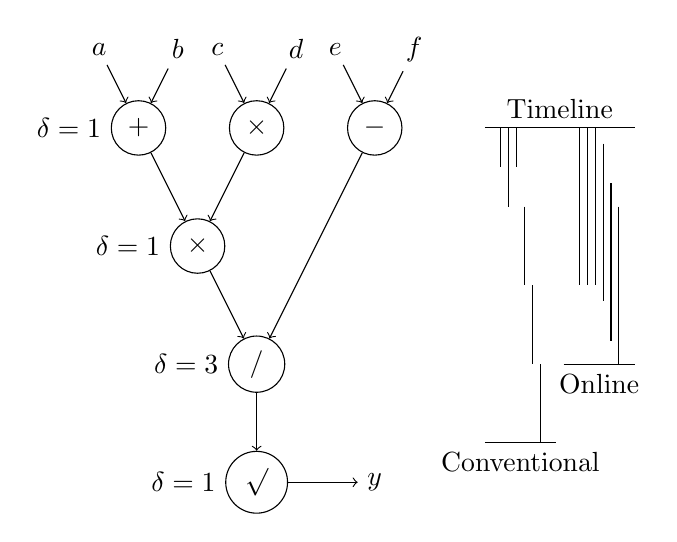
\begin{tikzpicture}
  \path
  (-0.5,5)   node(a) {$a$}
  (0.5,5)    node(b) {$b$}
  (1.0,5)    node(c) {$c$}
  (2,5)      node(d) {$d$}
  (2.5,5)    node(e) {$e$}
  (3.5,5)    node(f) {$f$}

  (0,4)      node[circle,draw,label=left:{$\delta=1$}](p1)  {$+$}
  (1.5,4)    node[circle,draw](p2)                          {$\times$}
  (3,4)      node[circle,draw](p3)                          {$-$}
  (0.75,2.5) node[circle,draw,label=left:{$\delta=1$}](p4)  {$\times$}
  (1.5,1)    node[circle,draw,label=left:{$\delta=3$}](p5)  {$/$}
  (1.5,-0.5) node[circle,draw,label=left:{$\delta=1$}](p6)  {$\surd$}

  (3,-0.5)   node(y) {$y$}
  ;

  \draw[->] (a) -- (p1);
  \draw[->] (b) -- (p1);
  \draw[->] (c) -- (p2);
  \draw[->] (d) -- (p2);
  \draw[->] (e) -- (p3);
  \draw[->] (f) -- (p3);

  \draw[->] (p1) -- (p4);
  \draw[->] (p2) -- (p4);
  \draw[->] (p3) -- (p5);
  \draw[->] (p4) -- (p5);
  \draw[->] (p5) -- (p6);

  \draw[->] (p6) -- (y);

  \draw (4.4,4) -- (6.3,4) node[midway,above]() {Timeline};;
  \draw (4.4,0) -- (5.3,0) node[midway,below]() {Conventional};
  \draw (5.4,1) -- (6.3,1) node[midway,below]() {Online};

  \draw (4.6,4) -- (4.6,3.5);
  \draw (4.7,4) -- (4.7,3);
  \draw (4.8,4) -- (4.8,3.5);
  \draw (4.9,3) -- (4.9,2);
  \draw (5.0,2) -- (5.0,1);
  \draw (5.1,1) -- (5.1,0);

  \draw (5.6,4) -- (5.6,2);
  \draw (5.7,4) -- (5.7,2);
  \draw (5.8,4) -- (5.8,2);
  \draw (5.9,3.8) -- (5.9,1.8);
  \draw (6.0,3.3) -- (6.0,1.3);
  \draw (6.1,3) -- (6.1,1);

\end{tikzpicture}
  \caption{Computing $y=\sqrt{(a+b)cd/(e-f)}$ with serial online operators~\cite{Ercegovac1}}
  \label{Online}
\end{figure}

As illustrated in figure~\ref{Online}, while each individual operation may take longer than its conventional counterpart, online arithmetic can provide a speedup if the operators are chained in serial.
In addition to the tradeoff in time, individual online arithmetic operators also uses more memory.
To perform all computation from the MSD to the LSD, the use of a redundant number system is compulsory.
However, this redundancy also has its advantage in making the operators scalable.
The time required per digit can be made independent of the length of the operands~\cite{Trivedi1}.

A recently proposed architecture allows the precision of online arithmetic to be controlled at runtime~\cite{Zhao1}.
Traditionally, this runtime control was restricted due to the parallel adders present in the multipliers and dividers.
This architecture reuses a fixed-precision adder and stores residues in on-chip RAM.
As such, a single piece of hardware can be used to calculate to any precision, limited only by the size of the on-chip RAM.

The way online arithmetic alleviates the second problem of fixed precision falls out directly from its MSD-first nature.
Suppose the output of a conventional ripple adder is sampled before it has completed its operation.
In this case, the lower digits would have been completed, but the carry would not have reached the higher ones.
This means the error on the result would be significant, as the top bits were still undetermined~\cite{Shi1}.
However, if the output of a parallel online adder is sampled before its completion, the lower bits would be the undetermined ones.
This means the error of the operation would be small.
With overclocking, online arithmetic operators fail gracefully, losing their precision gradually from the lowest bits first.
Thus, it allows for a runtime tradeoff between precision and frequency~\cite{Shi2}.

% REVISIT JD: find better arguments for high radix on FPGA for these two paras
\subsection{High-radix Arithmetic}
Conventional designs of arithmetic operators use binary representations.
The additional concerns of high-radix operators did not provide justifiable improvements as clock speed of processors kept increasing.
In recent years, the clock speed increase effectively ended, and semiconductor dies shrunk to extremely small sizes.
This means the relative processing time available in a clock period increased.
This enabled and drove the desire for accomplishing more per clock cycle, and high-radix arithmetic is one of them.
It has been shown that, high-radix offers power saving and/or reasonable speedups to the arithmetic operations~\cite{Catanzaro1}\cite{Amin1}\cite{Chen1}.

However, the savings are not without trade-offs.
If the radix chosen is not a power of 2, then this trade-off can become unfavourable if the specification requires much I/O and little computation.
This is because overhead of radix conversion would be significant~\cite{Whyte1}.
It is also unwise to use high-radix representations when the numbers are unusually small, thus making the savings offered by the high-radices negligible~\cite{Catanzaro1}.
The radix also cannot be too high, as the time in a clock period is still limited, if there is too many logic gates for the signal to propagate through, it might become the critical path and slow down the overall design.

The construct of FPGAs might make high-radices more attractive than it is on ICs.
As FPGAs contain small fast carry-ripple adders, high-radix adders may be able to exploit them to obtain significant speedups~\cite{Kornerup1}.

\subsection{High-radix Online Arithmetic}
Using high-radix number representations for online arithmetic is a relatively novel concept.
While there has been some research with similar premises~\cite{Lynch1}\cite{Lynch2}, We take a more direct approach with this project by implementing custom operators made for high-radix online arithmetic on an FPGA.
This will provide empirical results on the method, and will hopefully reveal practical insights along the way.

Furthermore, benchmarking this exotic arithmetic system with popular FPGA applications such as neural networks would be interesting, as there is not much precedence for it.


\begin{thebibliography}{1}
% Unused:
% M. D. Ercegovac and T. Lang. Digital Arithmetic



\bibitem{Brent1}
  R.P. Brent,
  ``\textit{A Regular Layout for Parallel Adders}'',
  \textit{IEEE Trans. Comput.}, vol. C-31, pp. 260-264,
  1982.

\bibitem{Catanzaro1}
  B. Catanzaro, and B. Nelson,
  ``\textit{Higher Radix Floating-Point Representations for FPGA-Based
  Arithmetic}'',
  \textit{Proceedings of the 51st Annual Design Automation Conference},
  2005.

\bibitem{Duncan1}
  R. Duncan,
  ``\textit{A Survey of Parallel Computer Architectures}'',
  \textit{Computer}, vol. 23, pp. 5-16,
  1990.

\bibitem{Duran1}
  J.W. Duran,
  ``\textit{An Evaluation of Random Testing}'',
  \textit{IEEE Trans. on Software Engineering}, vol. SE-10, no. 4, pp. 438-444,
  1984.

\bibitem{Ercegovac1}
  M.D. Ercegovac,
  ``\textit{On-line Arithmetic: An Overview}'',
  \textit{28th Annual Technical Symposium}, pp. 86-93,
  Internaltional Society for Optics and Photonics,
  1984.

\bibitem{Ercegovac2}
  M.D. Ercegovac, and T. Lang,
  ``\textit{Digital Arithmetic}'',
  Morgan Kaufmann,
  2003.

\bibitem{Hazwani1}
  S. Hazwani, et al,
  ``\textit{Randomness Analysis of Pseudo Random Noise Generator Using 24-bits
  LFSR}'',
  \textit{Fifth International Conference on Intelligent Systems, Modelling
  and Simulation},
  2014.

\bibitem{Lynch1}
  T. Lynch, and M.J. Schulte,
  ``\textit{A High Radix On-line Arithmetic for Credible and Accurate
  Computing}'',
  \textit{Journal of Universal Computer Science}, vol. 1, no. 7, pp. 439-453,
  1995.

\bibitem{Lynch2}
  T. Lynch, and M.J. Schulte,
  ``\textit{Software for High Radix On-line Arithmetic}'',
  \textit{Reliable Computing}, vol. 2, no. 2, pp. 133-138,
  1996.

\bibitem{Srinivas1}
  H.R. Srinivas, and K.K. Parhi,
  ``\textit{High-Speed VLSI Arithmetic Processor Architectures Using Hybrid
  Number Representation}'',
  \textit{J. of VLSI Sign. Process.}, vol. 4. pp. 177-198,
  1992.

\bibitem{Shi1}
  K. Shi, D. Boland, and G.A. Constantinides,
  ``\textit{Accuracy-Performance Tradeoffs on an FPGA through Overclocking}'',
  \textit{Proc. Int. Symp. Field-Programmable Custom Computing Machines},
  pp. 29-36,
  2013.

\bibitem{Shi2}
  K. Shi, D. Boland, E. Stott, S. Bayliss, and G.A. Constantinides,
  ``\textit{Datapath Synthesis for Overclocking: Online Arithmetic for
  Latency-Accuracy Trade-offs}'',
  \textit{Proceedings of the 13th Symposium on Field-Programmable Custom
  Computing Machines},
  pp. 1-6, ACM,
  2014.

\bibitem{Trivedi1}
  K.S. Trivedi, and M.D. Ercegovac,
  ``\textit{On-line Algorithms for Division and Multiplication}'',
  \textit{IEEE Trans. Comput.}, vol. C-26, no. 7, pp. 667-680,
  1977.

\bibitem{Whyte1}
  P. Whyte,
  ``\textit{Design and Implementation of High-radix Arithmetic Systems Based
  on the SDNR/RNS Data Representation}''
  \textit{Edith Cowan University},
  1997.

\bibitem{Zhao1}
  Y. Zhao, J. Wickerson, and G.A. Constantinides,
  ``\textit{An Efficient Implementation of Online Arithmetic}'',
  \textit{Int. Conf. on Field-Programmable Technology},
  2016.

% ------------------------------------------------------------------------------

\bibitem{Altera1}
  Altera Corporation,
  ``\textit{Cyclone V SoC Development Board Reference Manual}'',
  2015.
  % Available at:\\\url{www.intel.com/content/dam/www/programmable/us/en/pdfs/
  % literature/manual/rm_cv_soc_dev_board.pdf}.

\bibitem{Altera2}
  Altera Corporation,
  ``\textit{Memory System Design}'',
  \textit{Embedded Design Handbook},
  2010.
  % Available at:\\\url{www.intel.com/content/dam/www/programmable/us/en/pdfs/
  % literature/hb/nios2/edh_ed51008.pdf}.

\bibitem{Altera3}
  Altera Corporation,
  ``\textit{Introduction to Altmemphy IP}'',
  \textit{External Memory Interface Handbook: Reference Material}, vol. 3,
  2012.
  % Available at:\\\url{www.intel.com/content/dam/www/programmable/us/en/pdfs/
  % literature/hb/external-memory/emi_ddr3_ug.pdf}

\bibitem{Altera4}
  Altera Corporation,
  ``\textit{Phase-Locked Loop Basics, PLL},''.
  % Available at:\\\url{https://www.intel.com/content/www/us/en/programmable/
  % support/support-resources/operation-and-testing/pll-and-clock-management/
  % pll-basics.html}

\bibitem{Altera5}
  Altera Corporation,
  ``\textit{Creating Qsys Components}'',
  2018.
  % Available at:\\\url{https://www.intel.com/content/dam/www/programmable/us/
  % en/pdfs/literature/hb/qts/qsys_components.pdf}.

\bibitem{Altera6}
  Altera Corporation,
  ``\textit{Cyclone V Hard Processor System Technical Reference Manual}'',
  2018.
  % Available at:\\\url{https://www.intel.com/content/dam/www/programmable/us/
  % en/pdfs/literature/hb/cyclone-v/cv_54005.pdf}.

\bibitem{Imperial1}
  Imperial College
  ``\textit{An Ethics Code}'',
  \textit{Imperial College Research Ethics Committee},
  2013.

\bibitem{Intel1}
  Intel Corporation,
  ``\textit{Cyclone V SoC Development Kit and Intel SoC FPGA Embedded
  Development Suite}''.
  % Available at:\\\url{www.intel.com/content/www/us/en/programmable/products/
  % boards_and_kits/dev-kits/altera/kit-cyclone-v-soc.html}.

\bibitem{Intel2}
  Intel Corporation,
  ``\textit{Introduction to Intel FPGA IP Cores}'',
  2018.
  % Available at:\\\url{https://www.intel.com/content/www/us/en/programmable/
  % documentation/mwh1409960636914.html}.

\bibitem{Intel3}
  Intel Corporation,
  ``\textit{Avalon Interface Specifications}'',
  2018.
  % Available at:\\\url{https://www.intel.com/content/dam/www/programmable/us/
  % en/pdfs/literature/manual/mnl_avalon_spec.pdf}.

\bibitem{Rocket1}
  RocketBoards.org,
  ``\textit{GSRD 14.1 User manual}'',
  2015.
  % Available at:\\\url{https://rocketboards.org/foswiki/Documentation/GSRD141}.

\bibitem{Xilinx1}
  Xilinx, Inc,
  ``\textit{Zynq-7000 All Programmable SoC}'',
  2018.
  % Available at:\\\url{www.xilinx.com/support/documentation/
  % product-briefs/zynq-7000-product-brief.pdf}.

\bibitem{Xilinx2}
  Xilinx, Inc,
  ``\textit{ZedBoard (Zynq Evaluation and Development) Hardware User's Guide}'',
  2012.
  % Available at:\\\url{https://reference.digilentinc.com/_media/
  % zedboard:zedboard_ug.pdf}.
\end{thebibliography}

\end{document}